\documentclass{beamer}
\usetheme[progressbar=frametitle]{metropolis}          % Use metropolis theme

\graphicspath{{../src/images/}}

\usepackage{longtable}
\usepackage{pdfpages}	


% change progressbar thickness
\makeatletter
\setlength{\metropolis@titleseparator@linewidth}{1.5pt}
\setlength{\metropolis@progressonsectionpage@linewidth}{1.5pt}
\setlength{\metropolis@progressinheadfoot@linewidth}{2pt}
\makeatother

\usepackage{FiraSans}
\usepackage{makecell}
\usepackage{appendixnumberbeamer}

\title{Bezdrátová senzorová síť pro přístupový systém}
\date{25.6.2020}
\author{Bc. Tomáš Hyhlík}
\institute{Diplomová práce}
\begin{document}
  \maketitle

  

  %%%%%%%%%%%%%%%%%%%%%%%%%%%%
	\begin{frame}{Integrace WSN do architektury přístupového systému}

		\begin{figure}[h]
			\centering
			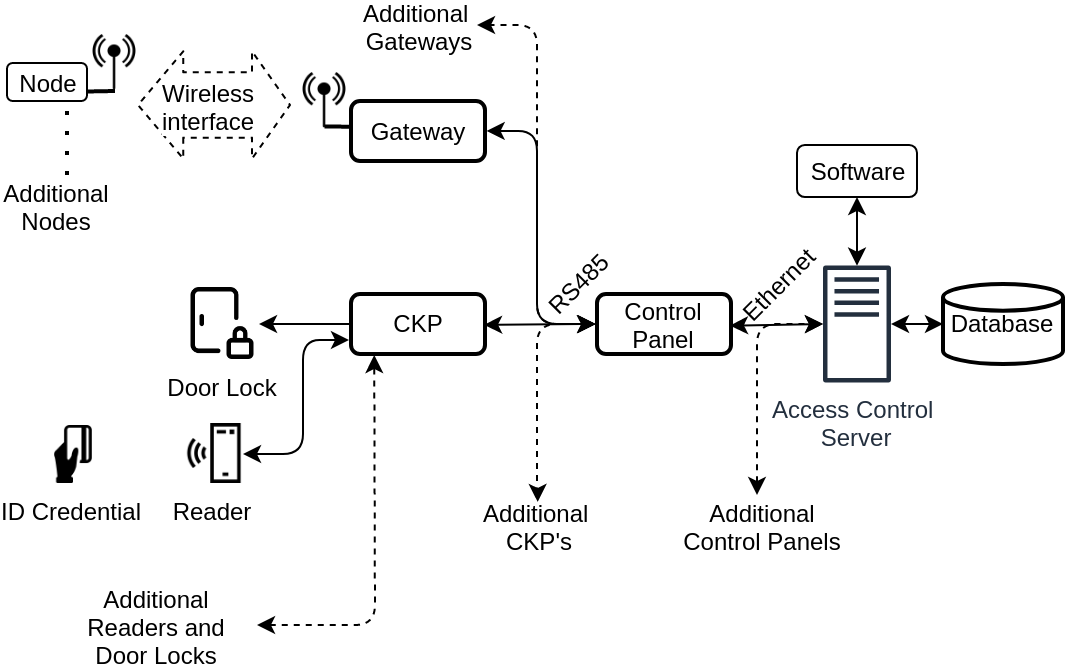
\includegraphics[width=1\textwidth]{ACS_IoT_extension_21}
			% \caption{Architektura přístupového systému firmy IMA s rozšířením o gateway senzorové sítě}
			\label{fig:ACS architecture IMA with geteway}
		\end{figure}
			
	\end{frame}



  %%%%%%%%%%%%%%%%%%%%%%%%%%%%
  \begin{frame}{Výběr bezdrátové technologie}

	Požadavky:
	\begin{itemize}
		\item Nízká cena HW
		\item Jednoduché přípojení koncových zařízení třetích stran (Third party)
		\item Velký počet dostupných koncových zařízení třetích stran na trhu 
		\item Jednoduchá implementace
		\item Nízká spotřeba energie koncových zařízení
	  \end{itemize}

  \end{frame}


  %%%%%%%%%%%%%%%%%%%%%%%%%%%%
  \begin{frame} {WSN gateway - HW}
	  
	\begin{figure}[!h]
		\centering
		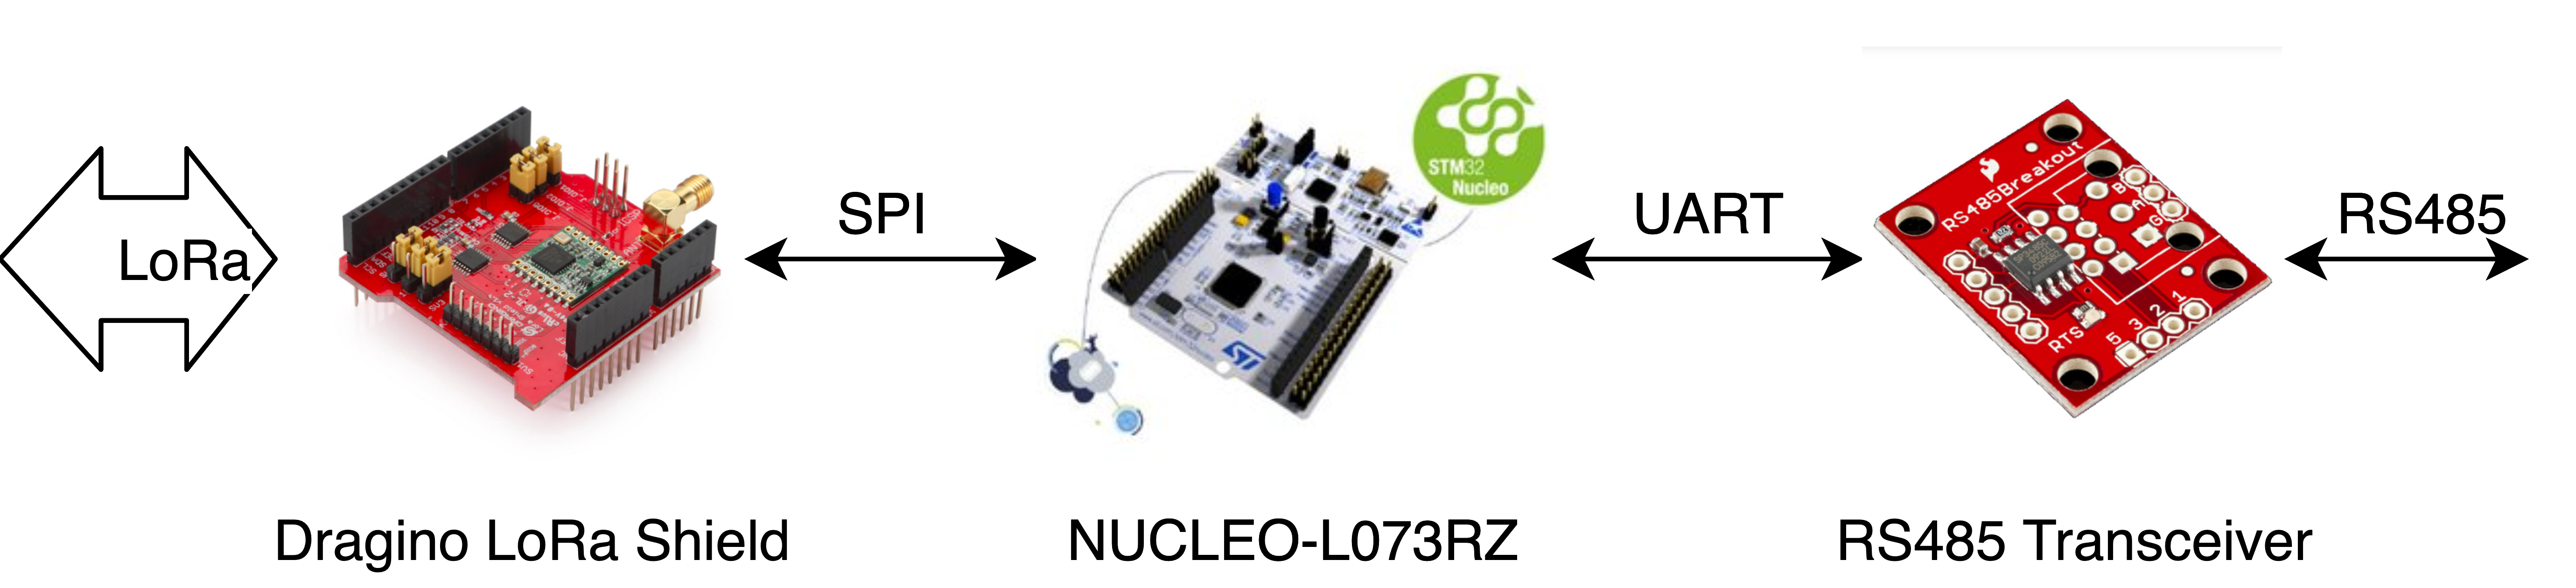
\includegraphics[width=1\textwidth]{LoRaWAN_gw_RS485_blockDiagram_3}
		% \caption{Blokový diagram navržené gatewaye senzorové sítě, Dragino LoRa Shield \cite{draginoWiki}, RS485 transceiver \cite{rs485tr}, NUCLEO-L073RZ \cite{nucleo-l073RZ_ST}}
		\label{fig:gatewayBlockDiagram}
	\end{figure}

  \end{frame}

  %%%%%%%%%%%%%%%%%%%%%%%%%%%%
  \begin{frame} {WSN gateway - SW}

	{\fontsize{9}{10}\selectfont 

		Rozdělení na nezávislé :
		\begin{itemize}
			\item LoRa
			\item LoRaWAN\_packet
			\item LoRa\_sensors
			\item rs485\_protocol
			\item usb
			\item eeprom
		\end{itemize}

		Dodatečné pomocné podprogramy
		\begin{itemize}
			\item buffer\_ring
			\item ByteArray
			\item LinkedList\_ByteArray
			\item aes (tiny-aes) \cite{lib_tiny-AES128-C} 
			\item cmac (openpana) \cite{lib_openpana}
		\end{itemize}
	}
  \end{frame}



  %%%%%%%%%%%%%%%%%%%%%%%%%%%%
  \begin{frame} {Testování dlouhodobého provozu}

	\begin{figure}[!h]
		\centering
		\includegraphics[width=1\textwidth]{5patro}
	\end{figure}

  \end{frame}


  %%%%%%%%%%%%%%%%%%%%%%%%%%%%
  \begin{frame} {Výpočet ...todo}

	{\fontsize{9}{9}\selectfont 
	\begin{equation}
		S_{MAX} = \frac{\frac{\frac{v_{485}}{B}}{l_{MAX}} - R}{P}
		\label{equ:max-count-of-sensors}
		\end{equation}
		
		kde:
		
		\begin{tabular}{l @{  } l}
		$v_{485}$ & rychlost přenosu dat v síti RS485 [bps]\\
		B        & počet bitů v bytu (pro přepočítání rychlosti přenosu dat na byty) \\
		$l_{MAX}$ & maximální délka paketu \\
		R        & rezerva rychlosti přenosu dat [\%]\\
		P        & počet paketů k přenesení dat z koncového zařízení \\
	\end{tabular}
	}

  \end{frame}


  %%%%%%%%%%%%%%%%%%%%%%%%%%%%
  \begin{frame} {}
	\begin{longtable} {|l|llll|}
		% % \footnotesize
		% \caption{Maximální počet připojených koncových zařízení v senzorové síti souběžně odesílající data skrze síť RS485 s určitou    
		% 	rezervou}      \label{tab:max-sensor-nodes} \\
		% 	\hline
		
			\textbf{RS485 rychlost přenosu dat} &       \multicolumn{4}{c|}{\textbf{Rezerva R}}	  	    \\
		
			$v_{485}$ {[bps]}  &	0 \%	&	10 \%	&	20 \%	&	30 \%  \\ \hline
		
			1200~~~ &    1	&    1	&    1	&    1 \\
			2400~~~ &    3	&    3	&    3	&    2 \\
			4800~~~ &    7	&    6	&    6	&    5 \\
			9600~~~ &   15	&   13	&   12	&   10 \\
			19200~~~ &   30	&   27	&   24	&   21 \\
			38400~~~ &   60	&   54	&   48	&   42 \\
			57600~~~ &   90	&   81	&   72	&   63 \\
			115200~~~ &  180	&  162	&  144	&  126 \\
			230400~~~ &  360	&  324	&  288	&  252 \\
			460800~~~ &  720	&  648	&  576	&  504 \\
			921600~~~ & 1440	& 1296	& 1152	& 1008 \\
			\hline
		
		\end{longtable}
		
		


  \end{frame}



%   \appendix
%   \begin{frame}{Reference}
  	
%   	 \bibliography{aeda_prezentace_bib}
% 	 \bibliographystyle{abbrv}
  	
%   \end{frame}

\end{document}